%%%%%%%%%%%%%%%%%%%%%%%%%%%%%%%%%%%%%%%%%
% Beamer Presentation
% LaTeX Template
% Version 1.0 (10/11/12)
%
% This template has been downloaded from:
% http://www.LaTeXTemplates.com
%
% License:
% CC BY-NC-SA 3.0 (http://creativecommons.org/licenses/by-nc-sa/3.0/)
%
%%%%%%%%%%%%%%%%%%%%%%%%%%%%%%%%%%%%%%%%%

%----------------------------------------------------------------------------------------
%	PACKAGES AND THEMES
%----------------------------------------------------------------------------------------

\documentclass[aspectratio=169]{beamer}
\usepackage[utf8]{inputenc}
\usepackage{booktabs}
\usepackage{graphicx}
\usepackage{array}
\usepackage{caption}
\usepackage{threeparttable}
\usepackage{lscape}
\usepackage{import}
\usepackage{amsmath}
\usepackage{csvsimple}
\usepackage{siunitx}
\usepackage{subfigure}
\usepackage{filecontents}
\newenvironment{wideitemize}{\itemize\addtolength{\itemsep}{10pt}}{\enditemize}
\usepackage{appendixnumberbeamer}
\usepackage{float}
\usepackage{amsmath}  
\usepackage{tikz,pgfplots}
\usepackage{tkz-fct}
\usepackage{amsthm}
\pgfplotsset{compat=1.10}
\usepgfplotslibrary{fillbetween}

\mode<presentation> {
\AtBeginSection[]
{
    \begin{frame}
        \frametitle{Table of Contents}
        \tableofcontents[currentsection]
    \end{frame}
}
% The Beamer class comes with a number of default slide themes
% which change the colors and layouts of slides. Below this is a list
% of all the themes, uncomment each in turn to see what they look like.

%\usetheme{default}
%\usetheme{AnnArbor}
%\usetheme{Antibes} -
%\usetheme{Bergen}
%\usetheme{Berkeley}
%\usetheme{Berlin}
\usetheme{Boadilla}
%\usetheme{CambridgeUS}
%\usetheme{Copenhagen} -
%\usetheme{Darmstadt}
%\usetheme{Dresden}
%\usetheme{Frankfurt}
%\usetheme{Goettingen}
%\usetheme{Hannover}
%\usetheme{Ilmenau}
%\usetheme{JuanLesPins}
%\usetheme{Luebeck}
%\usetheme{Madrid}
%\usetheme{Malmoe}
%\usetheme{Marburg}
%\usetheme{Montpellier}
%\usetheme{PaloAlto}
%\usetheme{Pittsburgh}
%\usetheme{Rochester} -
%\usetheme{Singapore}
%\usetheme{Szeged}
%\usetheme{Warsaw}

% As well as themes, the Beamer class has a number of color themes
% for any slide theme. Uncomment each of these in turn to see how it
% changes the colors of your current slide theme.

%\usecolortheme{albatross}
%\usecolortheme{beaver}
%\usecolortheme{beetle}
%\usecolortheme{crane}
%\usecolortheme{dolphin}
%\usecolortheme{dove}
%\usecolortheme{fly}
%\usecolortheme{lily}
%\usecolortheme{orchid}
%\usecolortheme{rose}
%\usecolortheme{seagull}
%\usecolortheme{seahorse}
%\usecolortheme{whale}
%\usecolortheme{wolverine}

%\setbeamertemplate{footline} % To remove the footer line in all slides uncomment this line
\setbeamertemplate{footline}[frame number] % To replace the footer line in all slides with a simple slide count uncomment this line
\setbeamertemplate{theorems}[numbered]
\setbeamertemplate{navigation symbols}{} % To remove the navigation symbols from the bottom of all slides uncomment this line
}
\setbeamertemplate{caption}{\raggedright\insertcaption\par}
  \setbeamertemplate{enumerate items}[default]
\usepackage{graphicx} % Allows including images
\usepackage{booktabs} % Allows the use of \toprule, \midrule and \bottomrule in tables
%\usepackage {tikz}
\newtheorem*{theorem*}{Theorem}
\newtheorem*{lemma*}{Lemma}
\newtheorem*{proposition}{Proposition}
\newtheorem*{corollary*}{Corollary}
\newtheorem*{definition*}{Definition}
\DeclareMathOperator*{\argmin}{arg\,min}
\newtheorem*{assumption}{Assumption}
\usetikzlibrary {positioning}
%\usepackage {xcolor}

%----------------------------------------------------------------------------------------
%	TITLE PAGE
%----------------------------------------------------------------------------------------

\title[Risk]{Lecture 1: Risk and Uncertainty} % The short title appears at the bottom of every slide, the full title is only on the title page

\author{Jacob Kohlhepp} % Your name
\institute[UCLA] % Your institution as it will appear on the bottom of every slide, may be shorthand to save space
{
Econ 101 \\ % Your institution for the title page
\medskip
}
\date{\today} % Date, can be changed to a custom date

\begin{document}

\begin{frame}
\titlepage % Print the title page as the first slide
\end{frame}

\begin{frame}{Introduction}
\begin{wideitemize}
    \item In Econ 11, we mostly assumed things were \textit{certain}.
    \begin{itemize}
        \item \textbf{Example:} Walrasian Eq. where Rosy has apples and Jamie has oranges and they each sell at a price. Everyone knows exactly how much they will enjoy apples or oranges.
    \end{itemize}
    \item But in reality many objects are not like this.
    \begin{itemize}
         \item \textbf{Example:} Used cars, insurance (I don't know if I will get into a car accident), lottery tickets, investments.
    \end{itemize}
    \item Our goal is to extend our toolbox so we can work with objects that are uncertain.
    \item Practical Applications: These tools are used broadly in finance, actuarial science and business.

\end{wideitemize}
    
\end{frame}

\begin{frame}{Notation, Terms, Definitions}
In this class:
    \begin{wideitemize}
            \item I denote lottery/gamble a as $X_a$, where $X_a$ is a random variable. So $a$ is the lottery, $X_a$ is the random variable representing lottery $a$.
            \item $E[X_a]$ always means expectation of $X_a$. 
            \item $Var(X_a)$ always means variance of $X_a$.
            \begin{itemize}
                \item It is often useful to recall this alternative formula for variance: $Var(X_a)=E[X_a^2]-E[X_a]^2$.
            \end{itemize}
            \item $log$ always means natural log (base e).
    \end{wideitemize}
\end{frame}
\begin{frame}{A Survey}
    Suppose you could enter one of three lotteries for free:
    \begin{wideitemize}
        \item[a.] $X_a$: \$100 with probability 50\%, \$0 with probability 50\%.
        \item[b.] $X_b$: \$49 with probability 100\%
        \item[c.] $X_c$: \$200 with probability 24\%, \$0 with probability 76\%.
    \end{wideitemize}
    Which would you choose? (Answer in the survey)
\end{frame}
 
 \begin{frame}{Risk Attitudes}
    \begin{wideitemize}
        \item Before looking at the results, notice some facts:
        \begin{itemize}
            \item b has lower expectation than a: $E[X_a]=50>49=E[X_b]$. 
            \item But a has higher variance than b: $Var(X_a)=2500>0=Var(X_b)$.
            \item So if you dislike variance or uncertainty, you will prefer a.
            \item $E[X_c]=48<49<50$. So in terms of expected money, c is worse than both a and b.
            \item However, the variance of c is higher: $Var(X_c) \approx 7296>2500>0$.
            \item You will only choose c if you like uncertainty/risk.
        \end{itemize}
        \item A rough interpretation of the results:
        \begin{itemize}
            \item If you chose b you are \textit{risk averse}: you dislike uncertainty/risk, and are willing to pay to reduce it.
            \item If you chose a you are either \textit{risk neutral} or slightly \textit{risk loving}.
            \item If you chose c you are \textit{risk loving.}
        \end{itemize}
    \item We can take these concepts and use a new tool to analyze them.
    \end{wideitemize}
\end{frame}
 
 \begin{frame}{Expected Utility Theory}
 \begin{wideitemize}
     \item We analyze uncertainty using \textbf{Expected Utility Theory.}
     \item Basically two things matter for decisions: \textbf{preferences over money} and \textbf{risk attitudes.}
     \item Main theorem:
     
     \begin{theorem}
Under a set of axioms (which you do not need to know), we can represent an individual's preferences over lotteries using an \textbf{expected utility function} $u$ where $E[u(X_a)] \geq E[u(X_b)]$ means that lottery $a$ is preferred to lottery $b$.
\end{theorem}

\item Main idea: We can represent risk attitudes using a utility function over money.

 \end{wideitemize}
 \end{frame}

\begin{frame}{Example}
Consider a person with expected utility function $u(x)=log(x+1)$. 
\begin{wideitemize}
    \item Given utility function we can compare any two lotteries over money by comparing $E[u(X_a)]$ and $E[u(X_b)]$.
    \item Lotteries can be discrete (like a coin flip) or continuous (like the exact temperature on a random day).
    \item If discrete, $E[X_A]=\sum_i f(x_i) x_i$ for pmf $f$.
    \begin{wideitemize}
        \item Example: For a lottery where you get 1 dollar for heads and 0 for tails: $E[X_{coin}] = 1\cdot 0.5 + 0 \cdot 0.5=0.5$
    \end{wideitemize}
    \item If continuous, $E[X_A]=\int xf(x)dx$ for pdf $f$.
    \item You will only be asked about discrete lotteries.
    \item \textbf{Exercise:} Let's rank the lotteries from the example.
\end{wideitemize}
\end{frame}

\begin{frame}{Risk Attitudes As Functions}
A person with expected utility function $u$ is...
\begin{wideitemize}
    \item \textbf{risk averse} if $u$ is concave.
    \item \textbf{risk neutral} if $u$ is linear.
    \item \textbf{risk loving} if $u$ is convex.
\end{wideitemize}

\end{frame}

\begin{frame}{Risk Attitudes As Functions}
    Which function is risk averse? Answer in the survey.
    \centering
    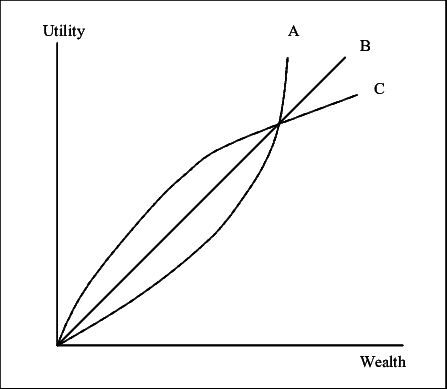
\includegraphics[width=0.5\textwidth]{Risk-Loving-A-Risk-Neutral-B-and-Risk-Averse-C-Utility-Curves.png}
    
    Source: Fleming et. al. (2003)
\end{frame}

\begin{frame}{Certainty Equivalent}

\begin{wideitemize}
    \item We often want to rank lotteries/gambles. The following concept is useful for ranking lotteries:
    \begin{definition}
    The amount of money for sure a decision maker is willing to pay for lottery $a$ is the \textbf{certainty equivalent} ($d_a$). Mathematically:
    \[u(d_a) = E[u(X_a)]\]
    \end{definition}
    \item Given a lottery that gives me $d$ dollars for sure and $X_a$, it is the value of d where I am indifferent.
    \item We can use this to rank lotteries. if $d_a>d_b$ then the decision maker prefers lottery a.
    \item We can also use this to calculate the willingness to pay for insurance.
    \pause \item Gut check: What is the certainty equivalent of a lottery a with $E[X_a]=10$ when the decision maker is risk neutral?
\end{wideitemize}
\end{frame}

\begin{frame}{Certainty Equivalents and Risk Attitudes}

Question: Given a lottery $X$, what can we say about the certainty equivalent of $X$ relative to $E[X]$ for a risk neutral person? A risk averse person? A risk loving person?
    
\end{frame}

\begin{frame}{Application: Insurance}
Consider a driver who faces monetary damages from driving given by a random variable $X$. The driver has wealth given by $w$ and has expected utility function $u(x)$.
\begin{itemize}
    \item We can think of these damages as a lottery $X$. Then the driver faces uncertain future wealth of $w-X$ (wealth less damages). This is the lottery they care about.
\end{itemize}

Suppose there is an insurance company which is risk neutral. This is reasonable because:
\begin{itemize}
    \item Insurance company cares about profits.
    \item Company will have many customers, so it cares about the average rather than the risk.
    \item More advanced explanation (not tested): by the Law of Large Numbers the sample average converges to expectation: $n^{-1}\sum_i X_i \to E[X]$, so with many customers uncertainty almost goes away.
\end{itemize}
\end{frame}

\begin{frame}{Application: Insurance}
\textbf{Question:} Suppose $u(x)=log(x)$, $w= \$10,000$, and the probability of an accident is $10\%$. if an accident happens, the driver incurs \$5,000 in damages. What is the certainty equivalent of the lottery the driver faces without insurance?

\begin{enumerate}
    \item \textbf{Define the problem.} The lottery $w-X$ is $\$10,000$ with probability $90\%$ and $10,000-5,000=\$5,000$ with probability $10\%$.
    \item The certainty equivalent is the amount the driver would take for sure that makes them indifferent between $w-X$. Call it d. d solves:
    \[E[u(w-X)]=u(d)\]
    \item Solving:
    \[E[log(w-X)]=0.1log(5000) + 0.9log(10000)=log(d)\]
    \[e^{9.1410}=9,330=d\]
\end{enumerate}

\end{frame}

\begin{frame}{Application: Insurance}
\textbf{Question:} Keep the same utility function and damage lottery. How much of a premium is the driver willing to pay for full insurance, where full insurance is defined as paying all the damages if there is an accident and 0 if there is no accident.

\begin{enumerate}
    \item \textbf{Define the problem.} Full insurance means that there is no uncertainty: wealth is constant in all states of the world, accident or not.
    \item \textbf{Write it in math.} Call the maximum premium $\tilde p$. The maximum premium the driver will pay is:
    \[u(10000-\tilde p)=E[u(w-X)]\]
    \item \textbf{Notice something clever.} Note that $10000-\tilde p$ is equal to the certainty equivalent. So we can either redo our work, or just solve:
    \[10000-\tilde p=9330\implies \tilde p = 670\]
    \item Try the long way for yourself to verify you get the same answer! Also feel free to do this again by switching up $X$ or the utility function.
\end{enumerate}

\end{frame}

\begin{frame}{Application: Insurance}
\textbf{Question:} Keep the same utility function and damage lottery. Think about the insurance company now. Define the actuarially fair premium to be the premium $p^*$ which makes expected profit 0 from full insurance. How much is the actuarially fair premium? What are the range of premiums under which both parties are willing to participate?

\begin{enumerate}
    \item \textbf{Define the problem.} Profit is $p-X$. We want to find $p^*$ that solves:
    \[E[\pi]=E[p-X]=0\]
    \item \textbf{Working it out:}
    \[E[p-X] = 0.1 (p^*-5000)+0.9p^* = p^*-500=0 \implies p^*=500\]
    \item The driver says yes when the premium is less than the $\tilde p$ we derived before. The insurance company says yes when the premium is above $p^*$. This gives a range of premiums which generate gains from trade:
    \[500=p^* < p < 670 = \tilde p \]
\end{enumerate}

\end{frame}

\begin{frame}{Exponential Utility}
\begin{wideitemize}
    \item In many settings, it is convenient to use a special family of utility function called exponential utility because it makes analysis easier.
    \item   It looks like this:
    
    \[u(x) = \frac{1-e^{-\theta x}}{\theta} \]
    where $\theta$ is a parameter capturing risk aversion. 
    
    \item When $\theta>0$ the decision maker is risk averse (a good exercise is to check this).
    
    \item When $\theta<0$ they are risk loving.
    
       \item What happens when $\theta \to 0$? Using L'Hopsital's rule:
       \[\lim_{\theta \to 0}  \frac{1-e^{-\theta x}}{\theta} = x\]
       So we have risk neutrality!
    
\end{wideitemize}
   
    
\end{frame}


\begin{frame}{Certainty Equivalent for Exponential Utility}
\begin{wideitemize}
    \item Why do we care about exponential utility?
    \item It has a nice expression for certainty equivalent when lotteries are normally distributed with mean $\mu$ and variance $\sigma^2$. The formula is:
    \[d = \mu - \theta \sigma^2/2\]
    \item You do not need to know how to get this. Just remember it.
    \item If you want to know, I derive it in the extra calculations section of these slides.
    \item But it has a nice interpretation: if $\theta>0$ (risk averse) an individual likes lotteries that give more on average (higher $\mu$) and dislikes lotteries that vary more (higher $\sigma^2$).
    
    \item Thus we can roughly ``measure risk" as the amount of variance.
\end{wideitemize}
    
\end{frame}

\begin{frame}{Application: Diversification (Challenging Example, Not Tested)}
    We will now use exponential utility with normal lotteries to see why you should ``diversify your portfolio." Suppose you have two independent stocks $a,b$ where $\mu_a=\mu_b$,$\sigma^2_a=\sigma^2_b$. What is the optimal amount you should invest in each stock?
    
    \begin{wideitemize}
        \item We use a trick: whatever lottery maximizes the certainty equivalent also maximizes utility (just like in Econ 11 taking logs doesn't matter)
        \item We want to maximize the certainty equivalent with respect to $a$.
        \[\max_a \mu_{portfolio} - \theta \sigma_{portfolio} ^2/2 \]
        \item Simplify and plug in $\mu_{portfolio}=\mu_a$ and $\sigma^2_{portfolio}=(1-2a+2a^2)\sigma_1^2$:
        \[\max_a \mu_a - \theta (1-2a+2a^2)\sigma_1^2\]
        \item Take FOC:
        \[-\theta\sigma_1^2(-2+4a)=0 \implies a = 1/2 \qquad \text{``Don't put all your eggs in one basket."}\]

    \end{wideitemize}
    
\end{frame}

\begin{frame}{}
    
\vspace{2cm}
\centering
\Large Extra Calculations

\end{frame}

\begin{frame}{Exponential Utility and Normal Lottery}
   \begin{enumerate}
        \item   When a lottery $X$ is normally distributed with mean $\mu$ and variance $\sigma^2$ it can be shown that:
    \[E[u(X)]=\theta^{-1} \bigg ( 1-e^{-\theta\mu+\theta^2 \sigma^2/2} \bigg )\]
    
       \item What is the certainty equivalent using this formula?
       \[u(d)=E[u(X)] \implies \frac{1-e^{-\theta d}}{\theta} = \theta^{-1} \bigg ( 1-e^{-\theta\mu+\theta^2 \sigma^2/2} \bigg )\]
       \[\implies e^{-\theta d} = e^{-\theta\mu+\theta^2 \sigma^2/2} \implies d = \mu - \theta \sigma^2/2\]
       So the certainty equivalent depends only on mean and variance. This is nice for finance and economic research.
       
    
   \end{enumerate}

    
\end{frame}

\begin{frame}{Portfolio with Two Assets}
     
    
    \begin{enumerate}
        \item 2 normal independent lotteries, $X_a, X_b$ with means $\mu_a, \mu_b$ and variances $\sigma^2_a, \sigma^2_b$.
        \item We have $\$1$ to invest total. Let $a$ be the amount we put in $a$ and $1-a$ be the amount we put in $b$. Call $X_p$ our portfolio form combining the assets.
        \item To get the expected value of the portfolio we just take the weighted average:
        \[\mu_p = a \mu_a + (1-a)\mu_b\]
        \item To get the variance of the portfolio we use the formula for the sum of variances:
        \[\sigma^2_p = a^2 \sigma^2_a + (1-a)^2\sigma^2_b\]
        \item We can now plug in our expressions for $\mu_p, \sigma^2_p$ into the certainty equivalent formula to get the certainty equivalent of the portfolio:
        \[d_p = \mu_p - \theta \sigma^2_p/2 = a \mu_a + (1-a)\mu_b -\theta (a^2 \sigma^2_a + (1-a)^2\sigma^2_b)/2\]
        \item When $\mu_a=\mu_b$ and $\sigma^2_a=\sigma^2_b$:
        \[d_p = \mu_p - \theta \sigma^2_p/2 = \mu_a -\theta (a^2 \sigma^2_a + (1-a)^2\sigma^2_a)/2=\mu_a -\theta \sigma^2_a(1-2a+2a^2)\]
    \end{enumerate}
    

    
\end{frame}
\end{document}

